\section{Background}

\subsection{The FaaS Function Communication Latency}
\label{subsec:faas-apps}

\begin{figure}
  \centering
  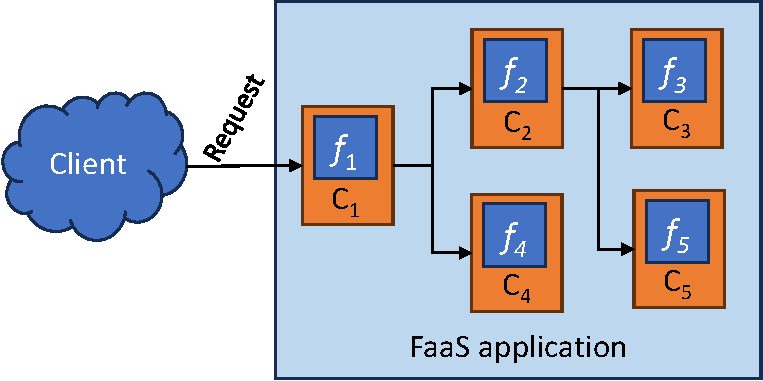
\includegraphics[width=\columnwidth]{figures/faas_application}
  \caption{\label{fig:faas-app} A schematic of a FaaS application conventionally deployed showing how an applicaiton is composed of multiple functions that each are hosted in their own container.}
\end{figure}

The FaaS computing model provides several advantages to the developer. One powerful advantage is hosting flexibility and that decisions about how to host an application is entirely left to the provider. This saves valuable developer time as managing hosting resources can be a demanding task. Furthermore, to unlock many of the advantages offered by the FaaS computing mode, FaaS applications need to be highly modular. This means that the functionality of a fully-fledged FaaS application should be backed by composing multiple smaller FaaS functions. While, in theory, a developer could choose to deploy a FaaS application consisting of only a single function containing all of the required functionality, this would relinquish many of the advantages that the FaaS model has to offer. Most notably, to patch or upgrade a single part of an application, the entire application would need to redeployed, a potentially risky operation. If the FaaS application was developed using a modular architecture consisting of several functions, the application can be updated function by function. Additionally, the loose coupling of FaaS functions means that a function can be written in any language at the discretion of the developer.

This modularity, however, comes with significant overheads. \Cref{fig:faas-app} shows a schematic of a common deployment scenario for a FaaS application. Each function, marked $f_{1..5}$ is hosted inside a separate container, marked $c_{1..5}$, and the communication between them is done using a network-backed RPC protocol. The use of a network-backed RPC interface in this case facilitates the loose coupling between functions. The main disadvantage, however, is that networked requests have high latency. In our example, whenever the first function $f_1$ in the FaaS application receives a request it subsequently calls its dependencies in order to perform its tasks. Since each inter-function call comes with the network overhead, examine, for example, the path from $f_1$ to $f_5$ in which we pay the RPC penalty twice. For complex FaaS applications, we therefore easily end up paying the RPC penalty multiple times to fulfill a request. Real-world applications can grow significantly more complex, in some cases containing more than 40 functions~\cite{gan19_open_sourc_bench_suite_micros}. Further, applications can perform multiple inter-function requests per operation which causes communication overheads to add up.

This strongly motivates the importance of mitigating this communication latency as the aggregated latencies in complex FaaS applications can quickly grow out of control, significantly harming the performance of real-world applications~\cite{gan19_open_sourc_bench_suite_micros}. Further, it is important to note that accessing the network layer is only strictly necessary for two functions running on different nodes. When possible, Providers prefer to schedule two functions on the same node in order to minimize their communication latency. In this case, using networked communication and thereby inducing the associated overhead is completely unnecessary.

\subsection{WebAssembly Components}
\label{subsec:wasm}

WebAssembly (Wasm)~\cite{rossberg22_webas_core_specif} is a portable bytecode format that originally targeted delivering high-performance compiled applications to web browsers. However, since none of Wasm's features explicitly targets web pages, it is also suitable as a general purpose bytecode format. The introduction of the WebAssembly System Interfaces (WASI) gives Wasm POSIX-like capabilities and allows Wasm programs to run outside the browser. A particularly appealing property of Wasm is the increasingly large number of programming languages that supports it as a target.

The WebAssembly Component Model \cite{compmodel} is a recent addition to the Wasm ecosystem that turns a compiled Wasm module into a portable, embedded and composable \emph{component} with a formally defined external API. A goal of the component model is therefore to allow developers to build language-independent applications that are composed several isolated components.

Following this definition, it becomes clear that the scope and purpose of a Wasm Component in this regard is the same as a FaaS function. The Wasm Component mode; even comes with its own dedicated IDL, known as WebAssembly Interface Types (WIT). A key observation, in this regard, is that IDL's that are used to specify the interfaces of FaaS functions, such as Protobuf for gRPC, are easily mapped to WIT.

Currently programs compiled from Rust, C/C++, Go and Java are supported by the Wasm component model, but there is no limitation that prevents further languages from being supported~\cite{bindgen}.


%%% Local Variables:
%%% mode: latex
%%% TeX-master: "main"
%%% TeX-command-extra-options: "-shell-escape"
%%% End:
